\documentclass[12pt,a4paper]{article}
\usepackage[dutch]{babel}
\usepackage[utf8]{inputenc}
\usepackage[margin=0.5in]{geometry}
\usepackage{amsmath}
\usepackage{amsfonts}
\usepackage{amssymb}
\usepackage{graphicx}
\usepackage{listings}
\usepackage{float}
\usepackage{hyperref}
\usepackage{color}



\begin{document}
\graphicspath{{images/}}
\DeclareGraphicsExtensions{.pdf,.png,.jpg}
\lstset{language=bash}
\author{Frank Willemsen}
\title{Een programma installeren met Synaptic}
\date{\today}
\maketitle
\abstract{\noindent Een beknopte inleiding tot het gebruik van Synaptic op Debian}
\section{Een programma installeren met Synaptic.}


Je opent Synaptic. Dit programma vind je waarschijnlijk onder Overige. Zo niet, dan kun je altijd \emph{Opdracht uitvoeren\ldots} kiezen uit het startmenu en dan ``Synaptic'' invoeren. 

\begin{figure} [H]
\centering
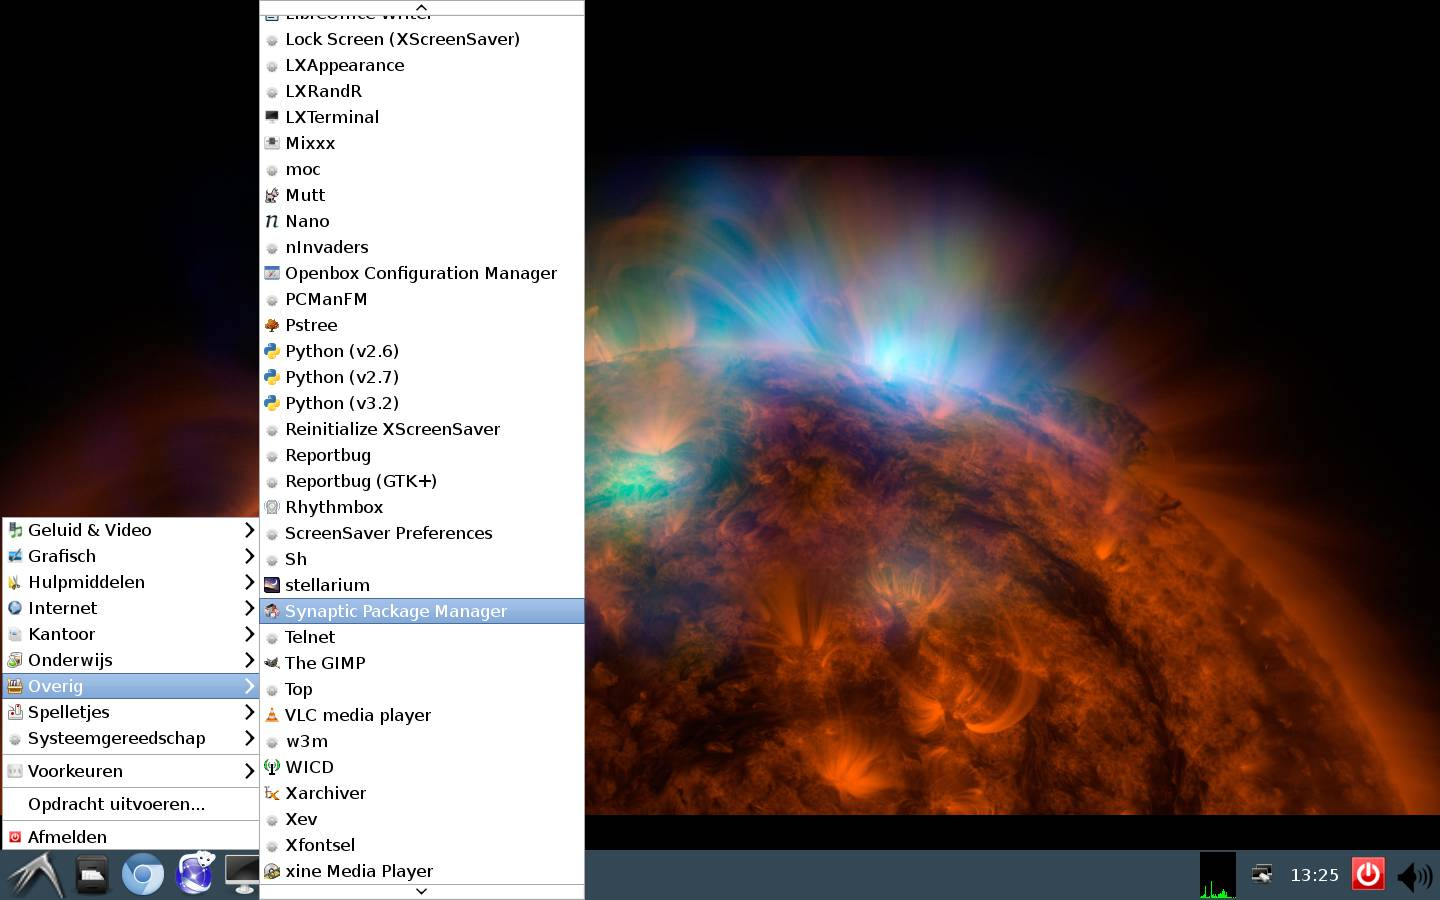
\includegraphics[width=0.6\textwidth]{plaatje01}
\caption{open Synaptic}
\label{plaatje01}
\end{figure}

\noindent Synaptic vraagt gelijk bij openen naar je wachtwoord. Het heeft dit nodig om software te kunnen installeren of te verwijderen.

\begin{figure} [H]
\centering
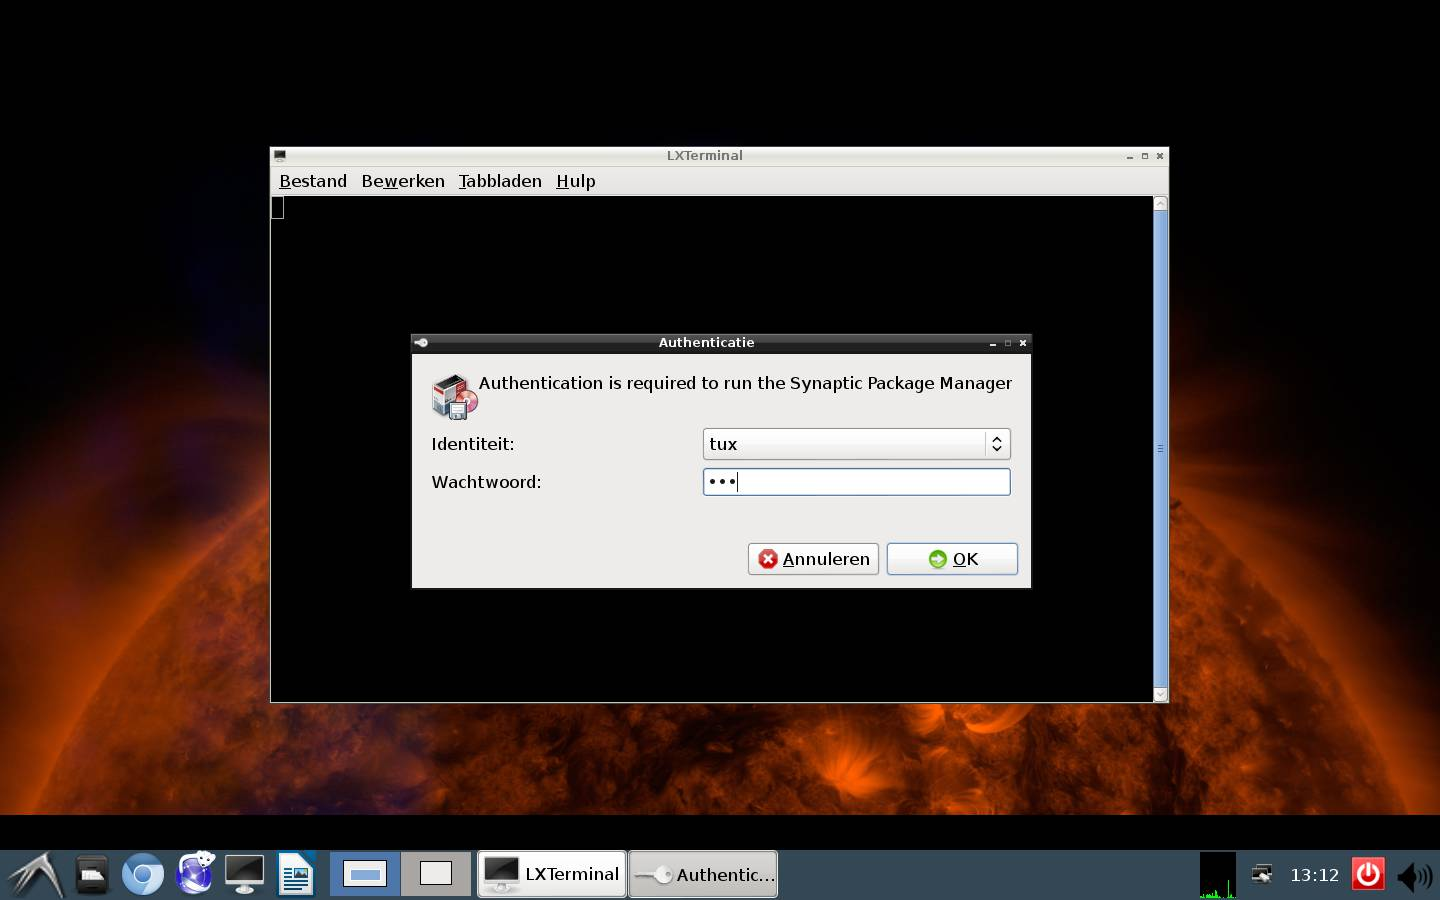
\includegraphics[width=0.6\textwidth]{plaatje02}
\caption{Wachtwoordinvoer}
\label{plaatje02}
\end{figure}

\clearpage

\noindent Nu je er toch bent, is het een goed idee om te herladen. Daarna weet je zeker dat je van alle programma's de nieuwste beschikbare versie kunt krijgen.

\begin{figure} [H]
\centering
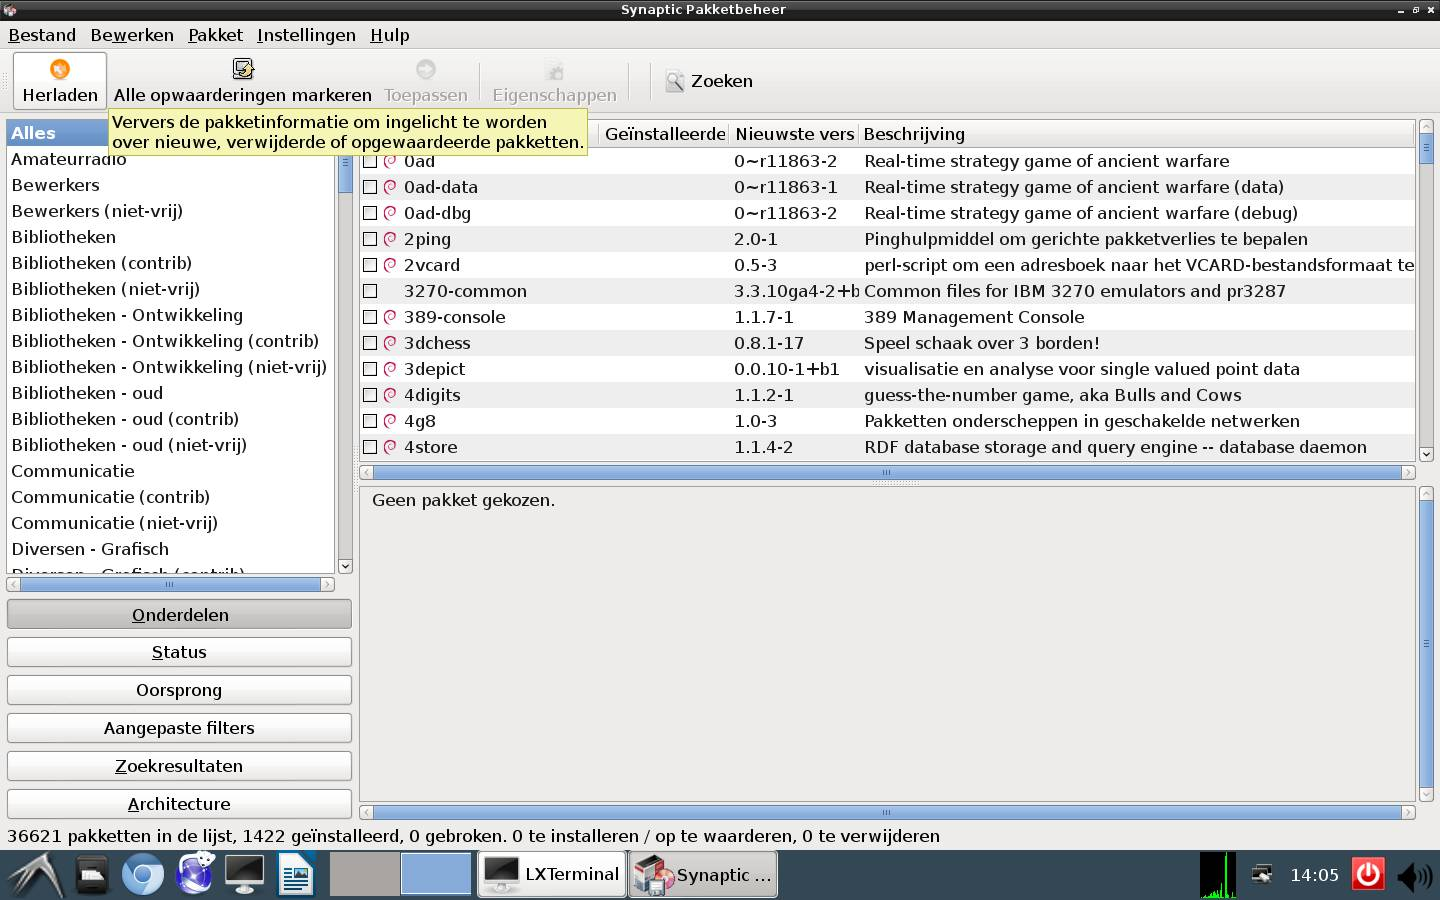
\includegraphics[width=0.45\textwidth]{plaatje04}
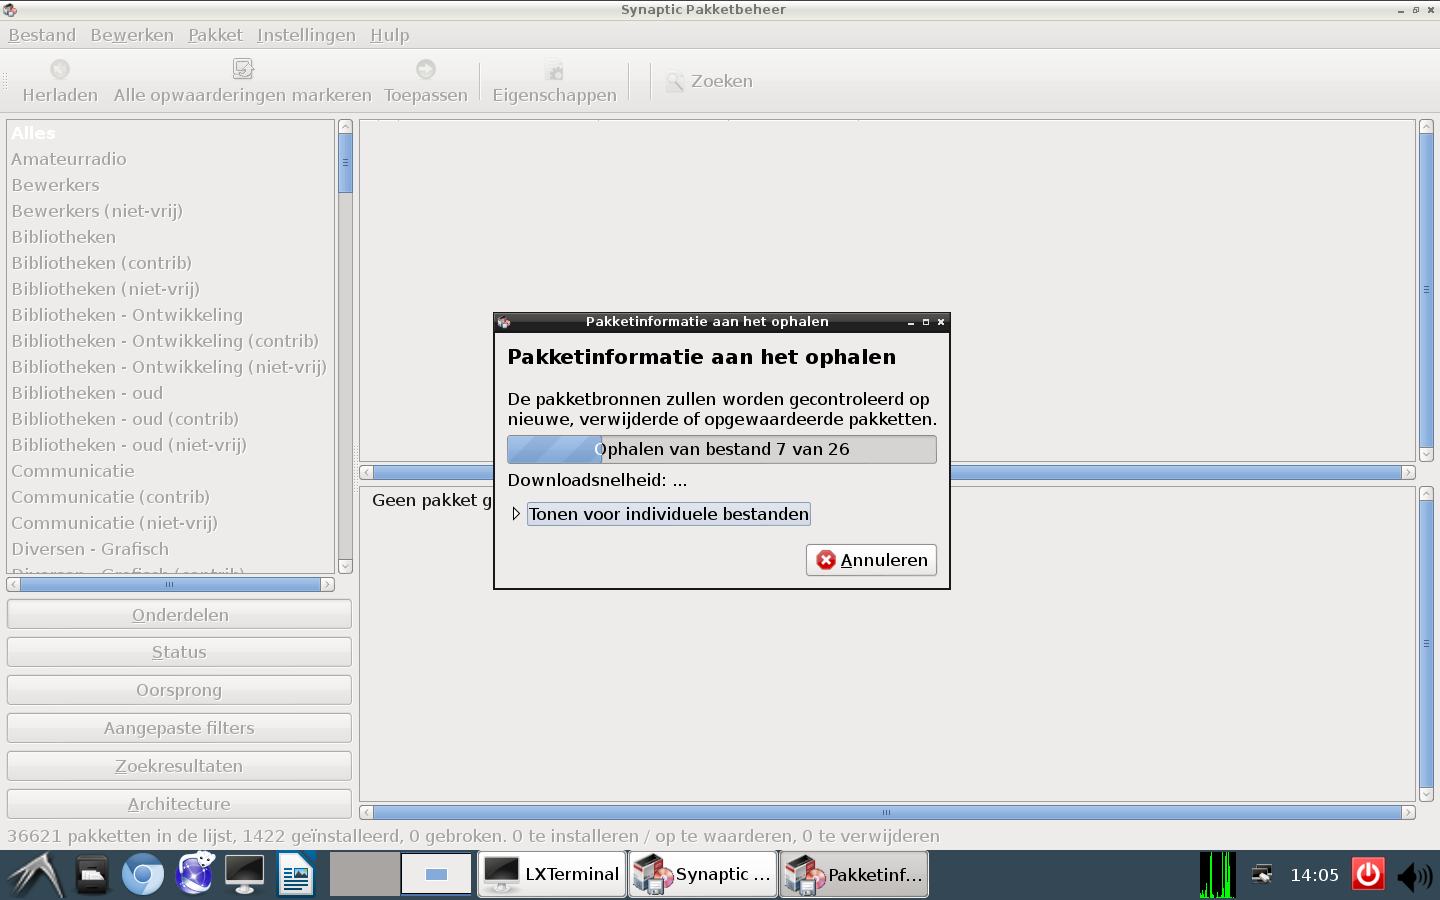
\includegraphics[width=0.45\textwidth]{plaatje05}
\caption{Pakketinformatie herladen}
\label{plaatje04}
\end{figure}

\noindent Als je weet welk programma je wilt installeren, hoef je niet moeilijk te doen en het in een menu op te zoeken. Je doet Zoeken en voert de naam in.

\begin{figure} [H]
\centering
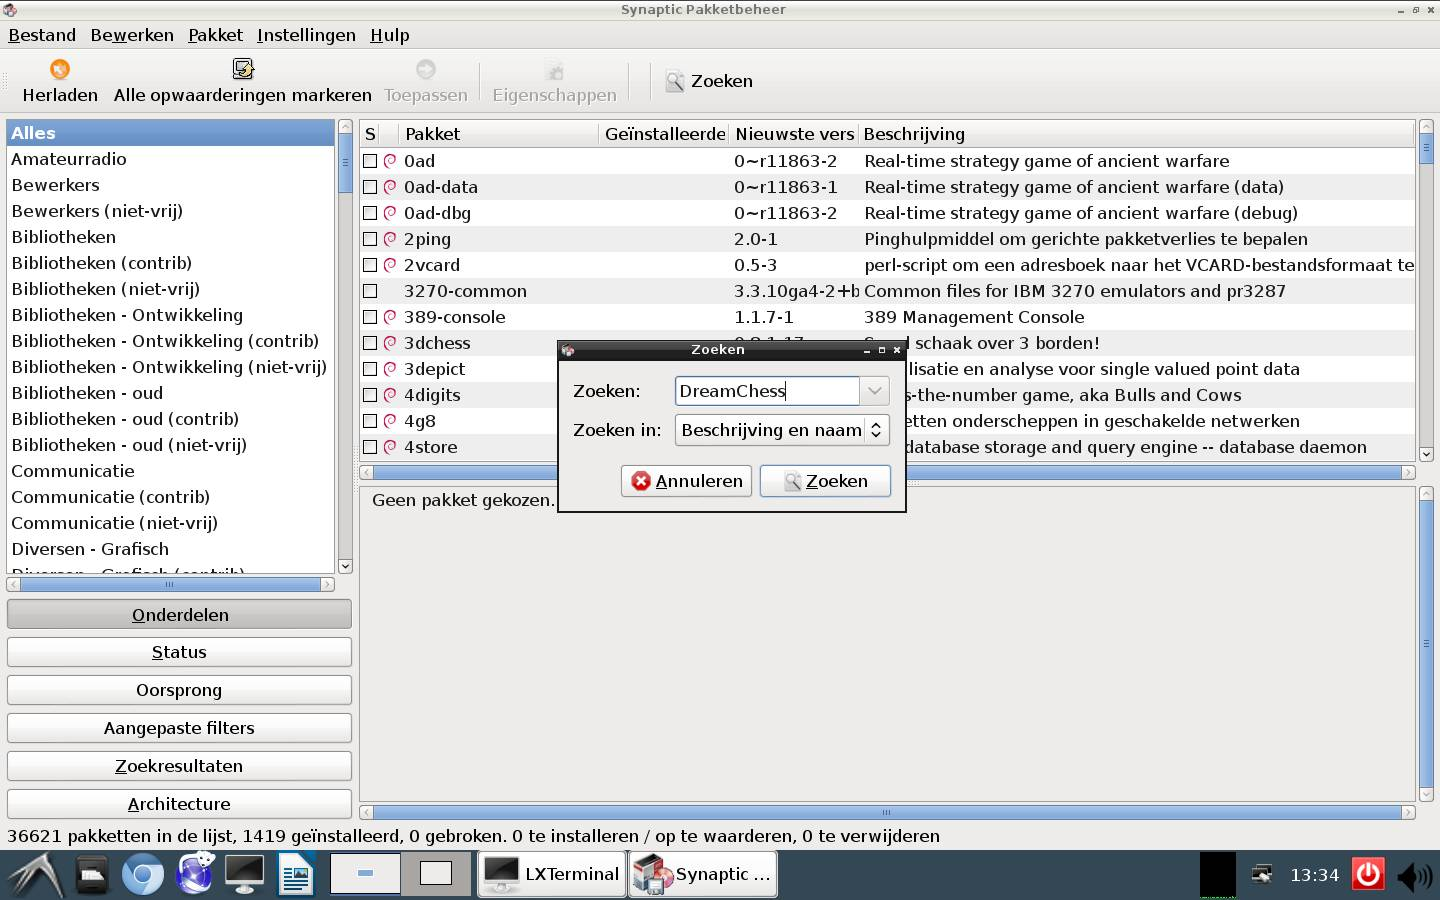
\includegraphics[width=0.6\textwidth]{plaatje06}
\caption{Zoeken naar een programma}
\label{plaatje06}
\end{figure}

\noindent In dit voorbeeld installeren we het schaakspelletje DreamChess. Dat vink je aan.	

\begin{figure} [H]
\centering
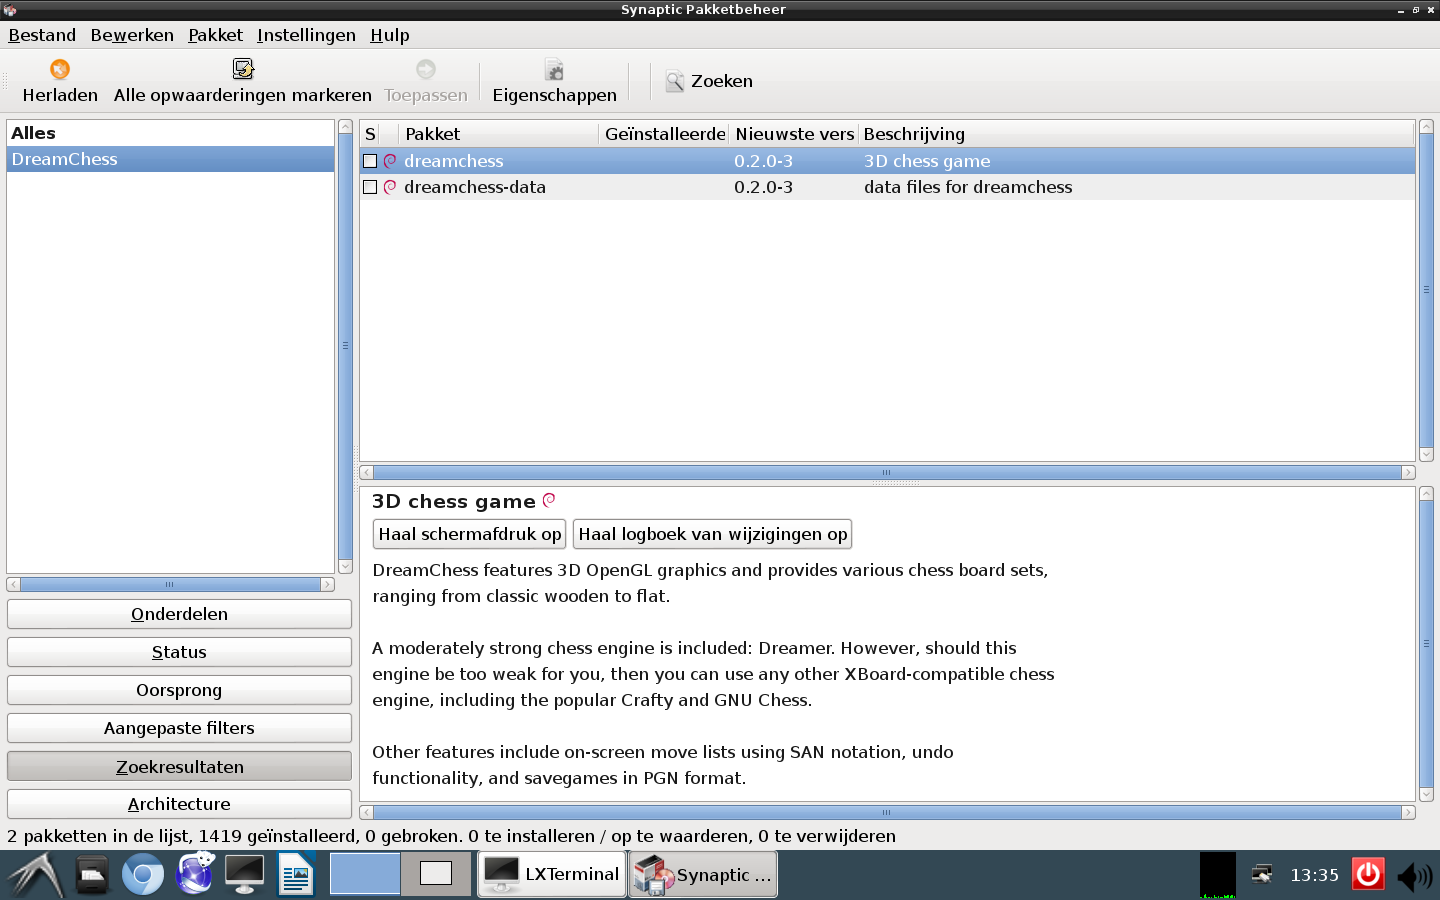
\includegraphics[width=0.6\textwidth]{plaatje07}
\caption{Selectie}
\label{plaatje07}
\end{figure}

\clearpage

\noindent DreamChess vraagt je om nog een paar andere stukjes software aan te vinken. Het functioneert niet naar behoren zonder. Dus klik je Markeren.

\begin{figure} [H]
\centering
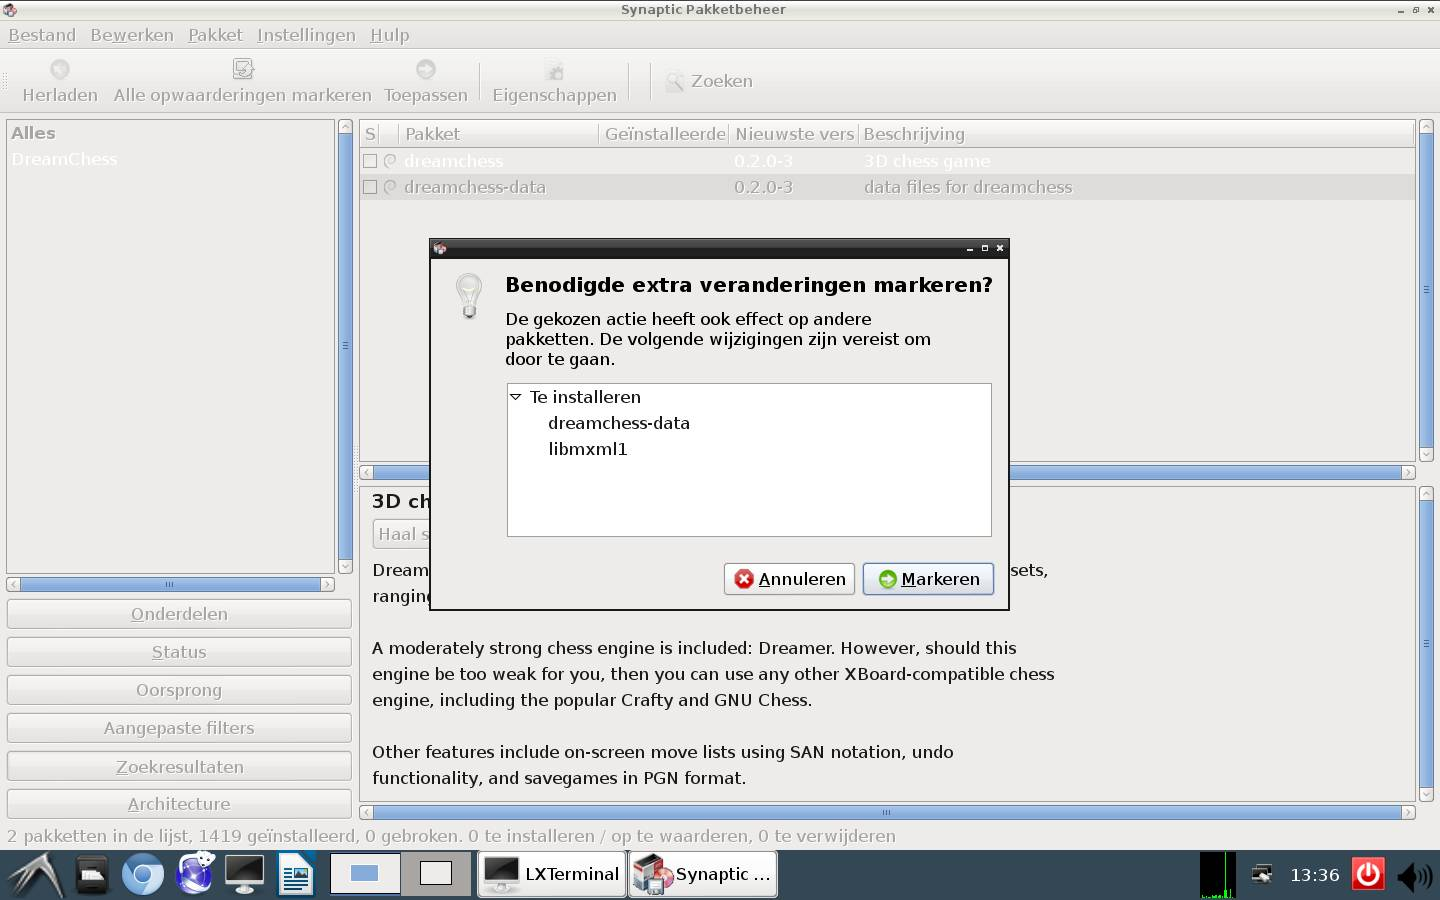
\includegraphics[width=0.6\textwidth]{plaatje08}
\caption{Benodigde extra software}
\label{plaatje08}
\end{figure}

\noindent Nu klik je Toepassen. Er wordt nog eens gevraagd of je zeker weet dat je dit wilt doen. Dus klik je opnieuw op Toepassen. 

\begin{figure} [H]
\centering
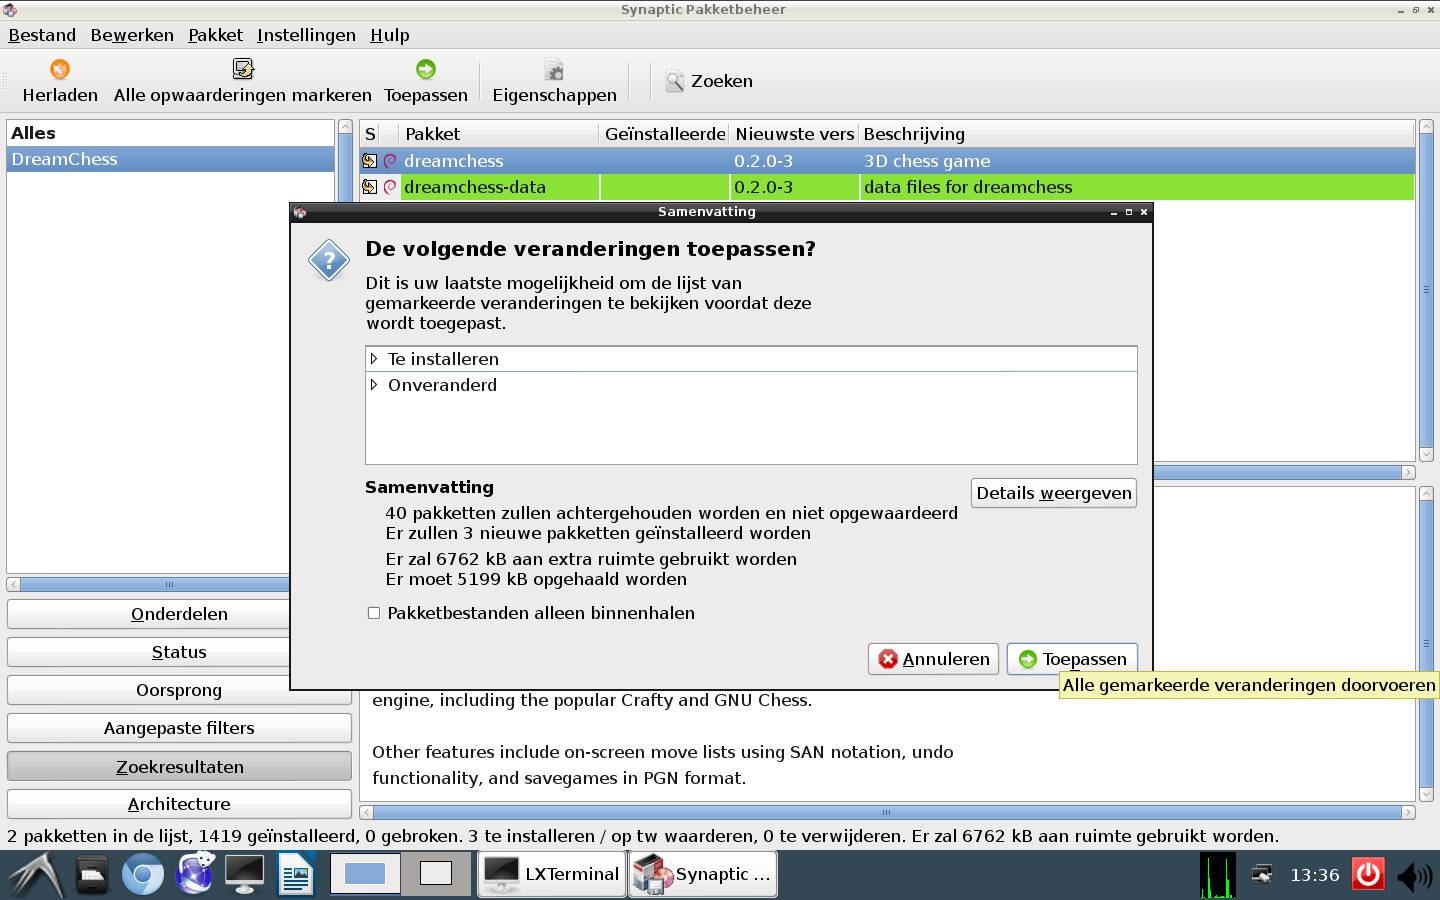
\includegraphics[width=0.6\textwidth]{plaatje10}
\caption{Kies Toepassen om je keus te bevestigen}
\label{plaatje10}
\end{figure}

\noindent Synaptic gaat nu softwarepakketten ophalen. Daarna gaat het deze installeren.

\begin{figure} [H]
\centering
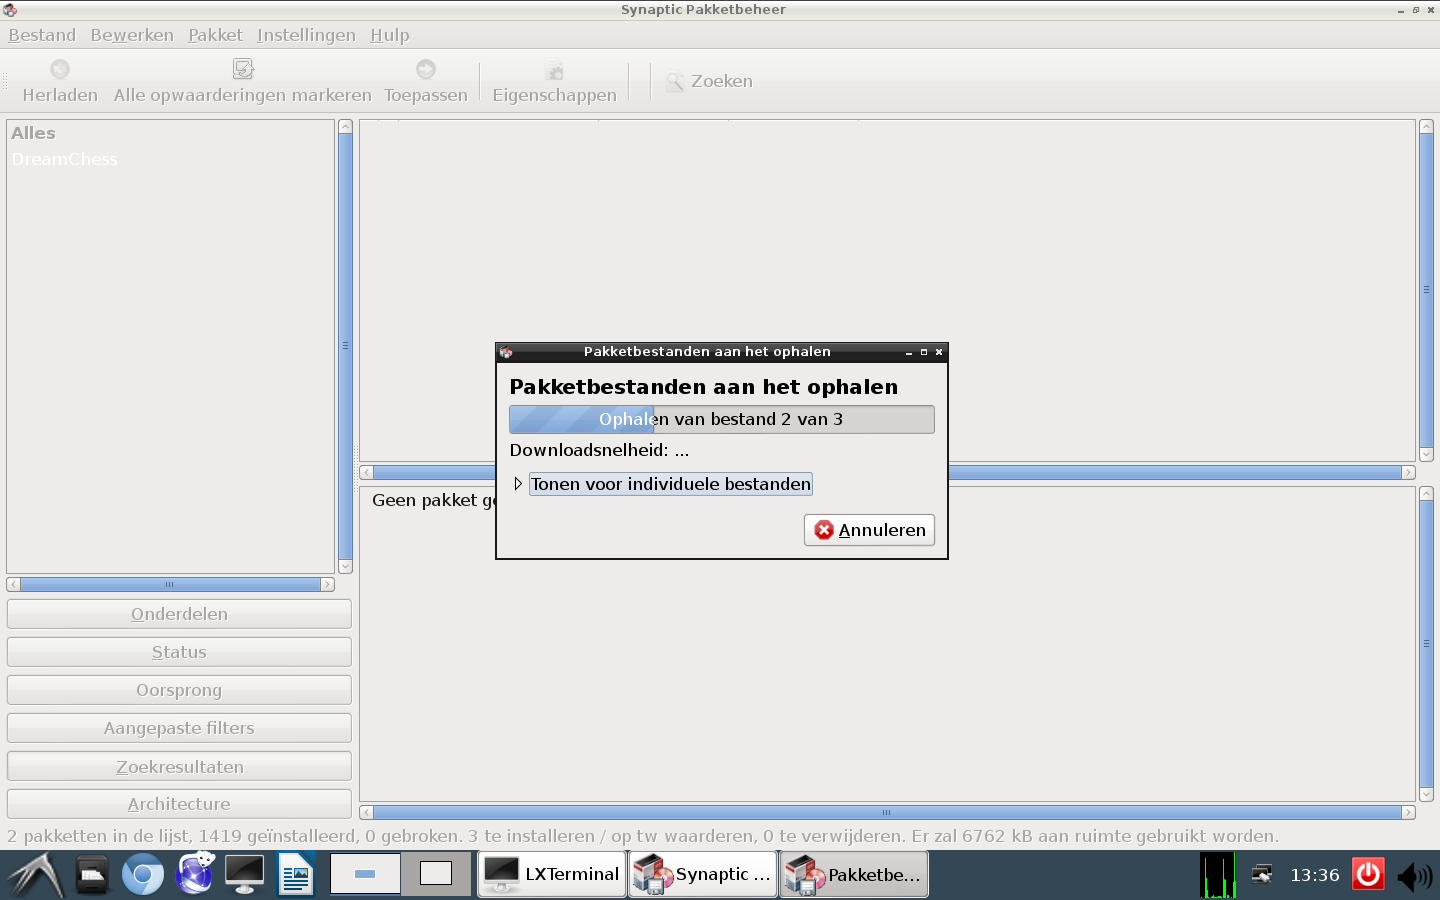
\includegraphics[width=0.45\textwidth]{plaatje11}
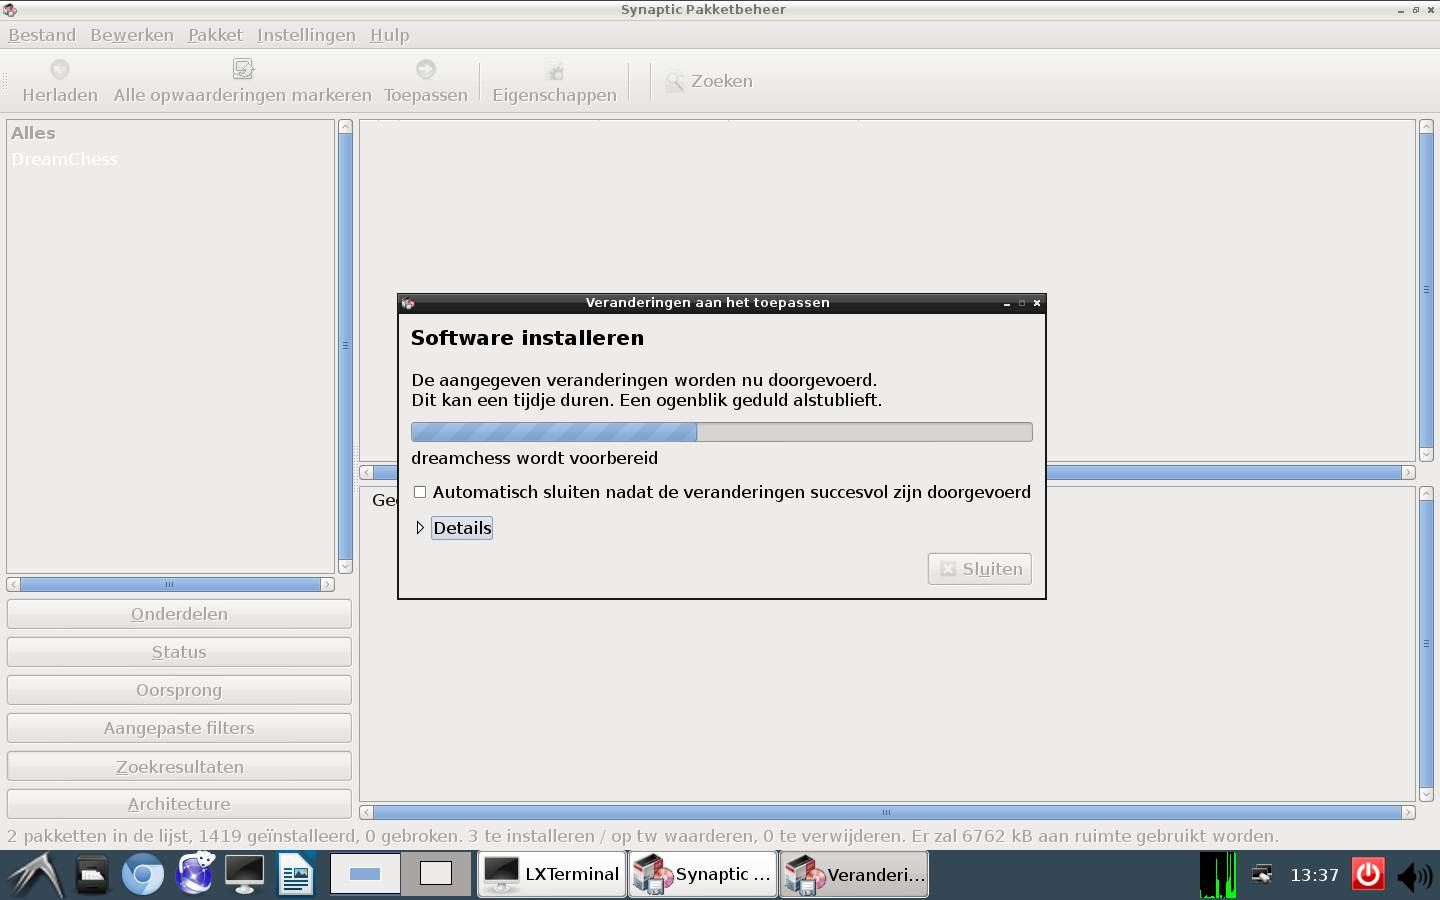
\includegraphics[width=0.45\textwidth]{plaatje12}
\caption{Download en installatie}
\label{plaatje11}
\end{figure}

\clearpage

\noindent Als het geslaagd is, kun je daarna Synaptic afsluiten.

\begin{figure} [H]
\centering
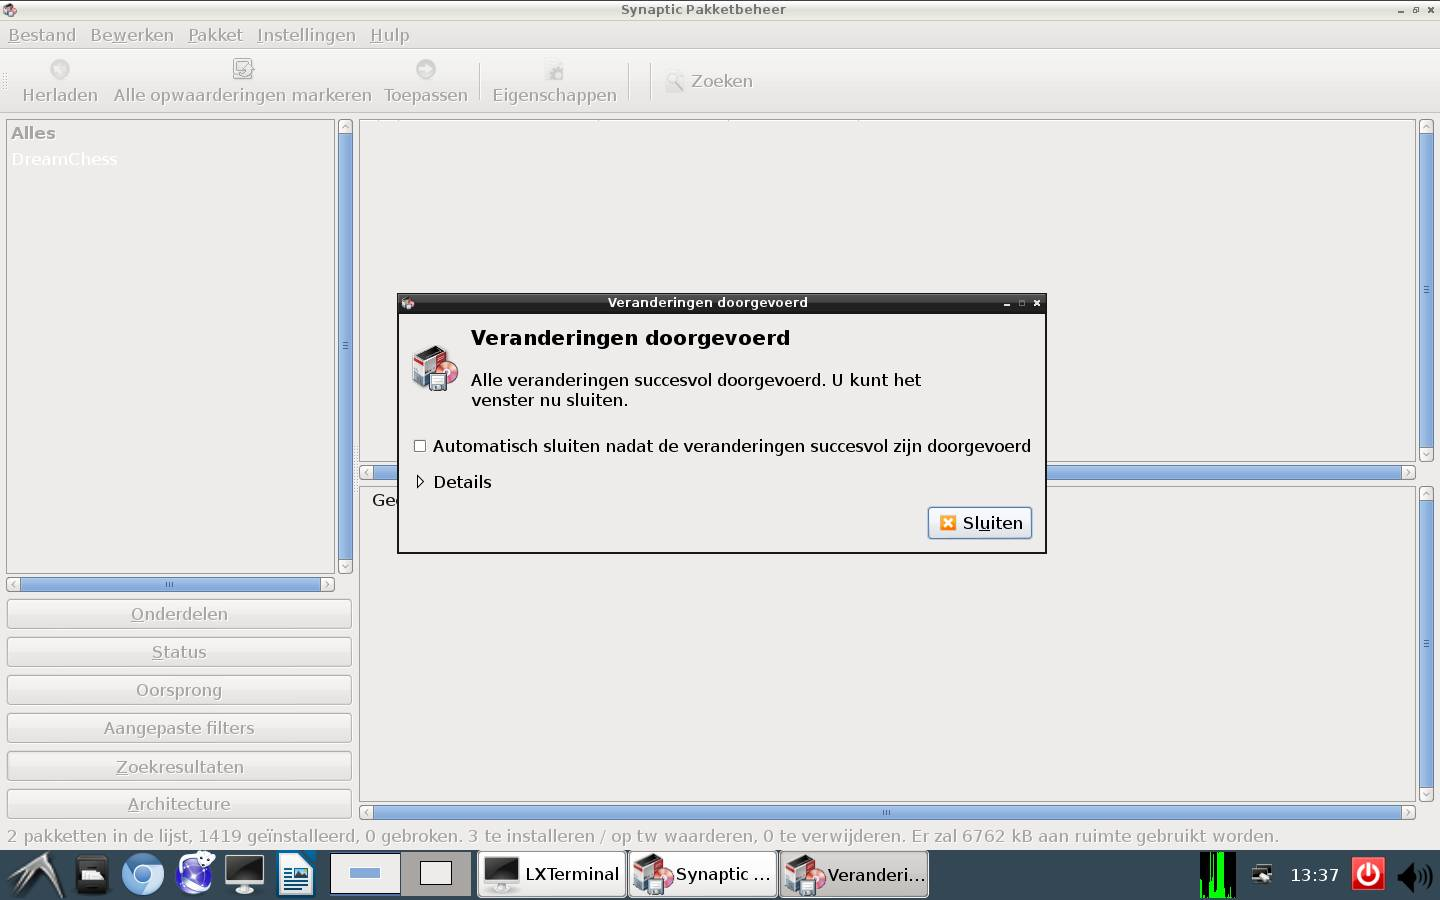
\includegraphics[width=0.6\textwidth]{plaatje13}
\caption{Klaar!}
\label{plaatje13}
\end{figure}

\noindent In Debian blijkt Dream Chess ondergebracht te zijn onder Spelletjes. We zijn klaar voor een potje schaak!

Mocht je het niet gelijk kunnen terugvinden, kies dan \emph{Opdracht uitvoeren\ldots} uit het startmenu en voer ``DreamChess'' in.

\begin{figure} [H]
\centering
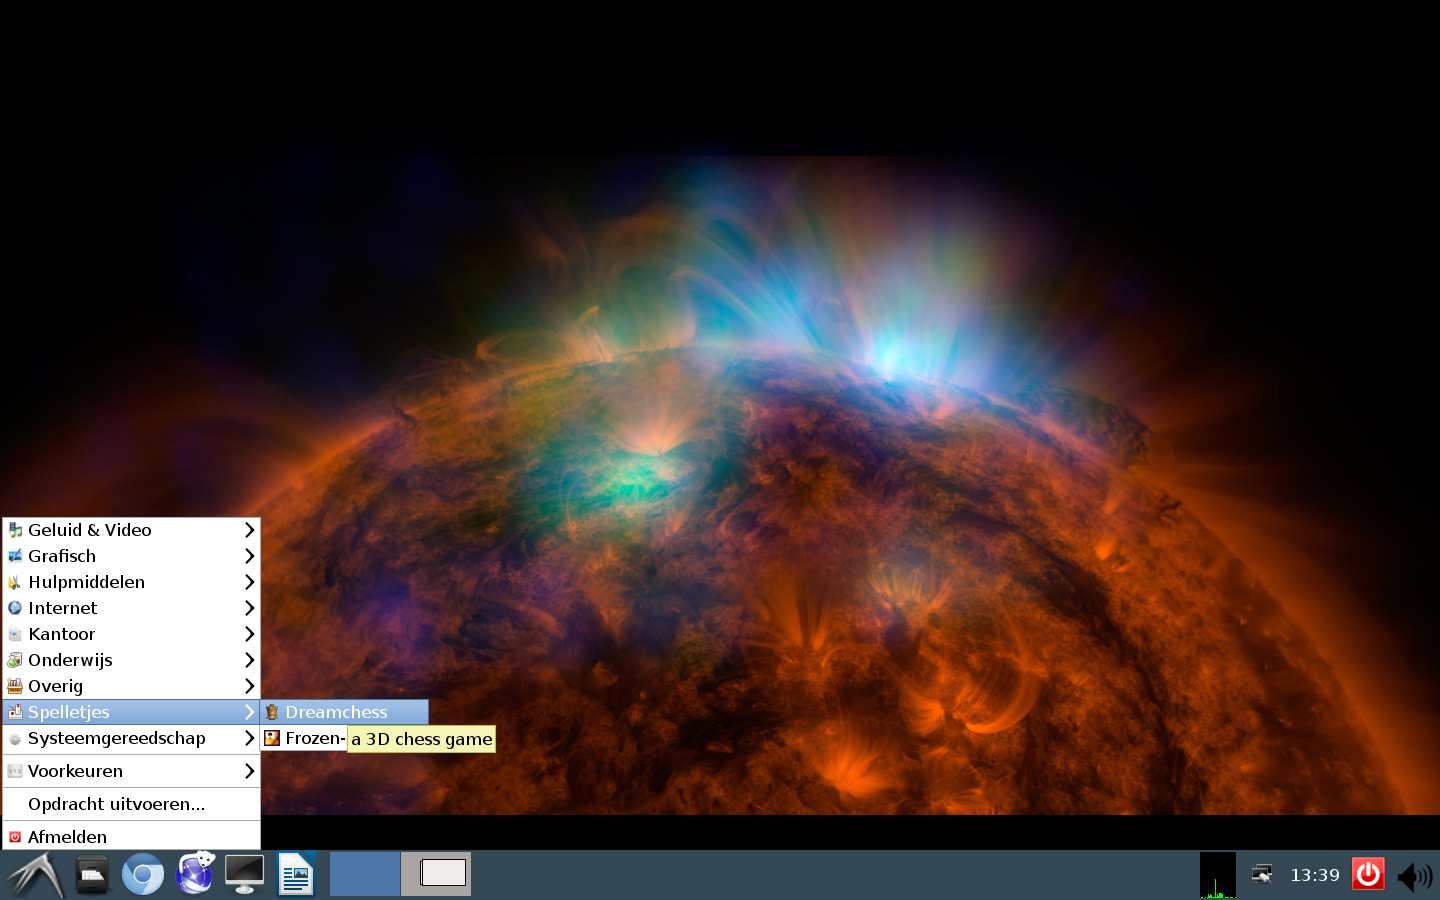
\includegraphics[width=0.45\textwidth]{plaatje14}
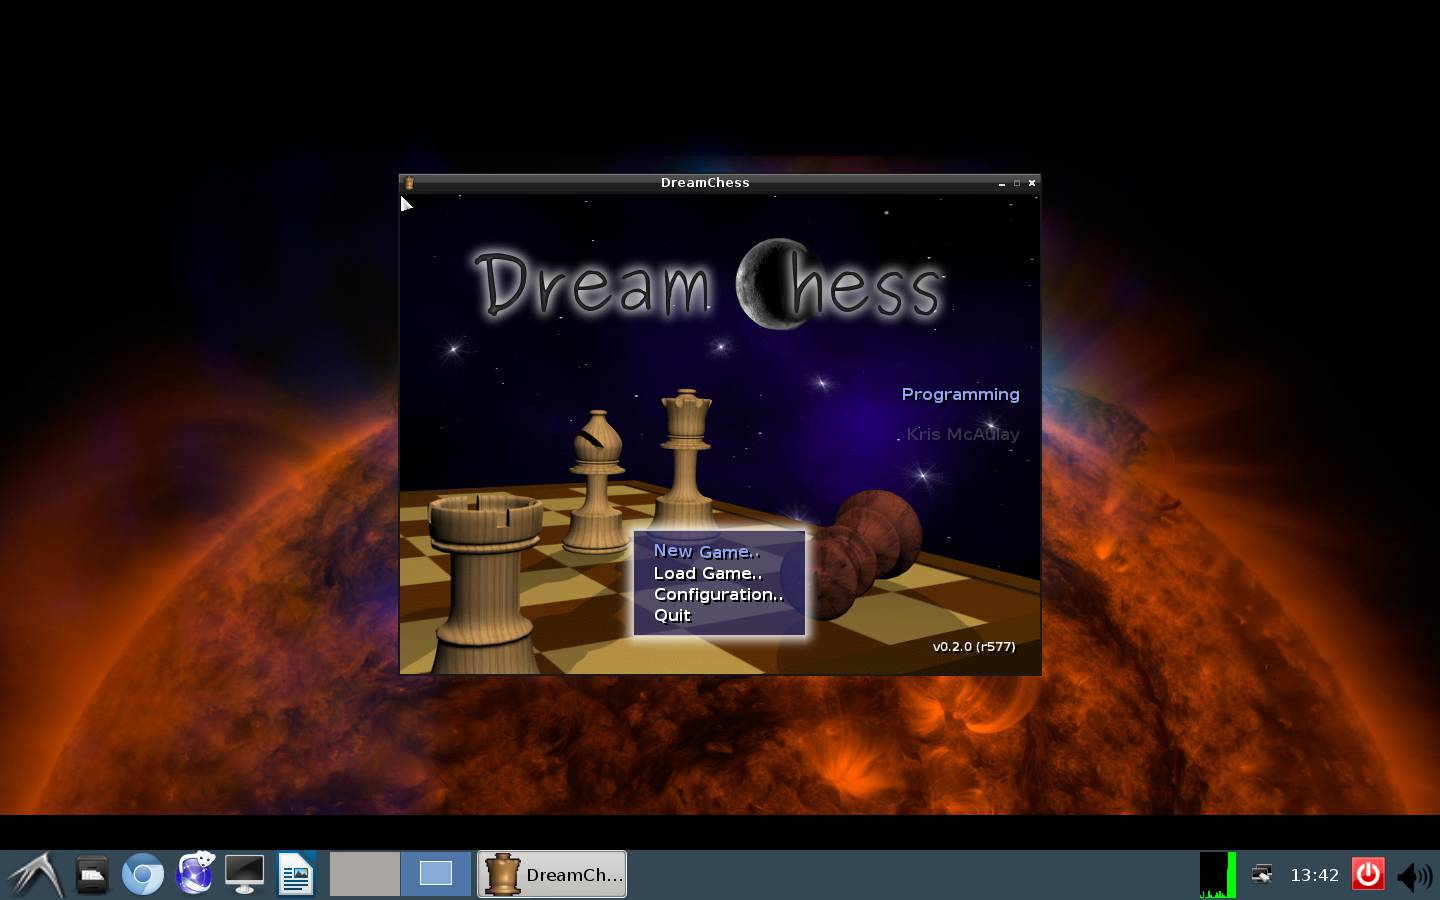
\includegraphics[width=0.45\textwidth]{plaatje15}
\caption{DreamChess is ge\"{i}nstalleerd}
\label{plaatje14}
\end{figure}

\clearpage

\section{Een programma de\"{i}nstalleren met Synaptic}

Stel, DreamChess was toch niet wat je ervan verwachtte. Dan de\"{i}nstalleer je het toch weer?

Dus open je Synaptic en zoek je op de zoekterm \emph{DreamChess}, zoals beschreven in het eerste deel van deze handleiding. 

In de pakkettenlijst staan nu nog maar twee pakketten: \emph{dreamchess} en \emph{dreamchess-data}. DreamChess kun je sowieso verwijderen. Dreamchess-data kan in dit geval ook, want we weten dat DreamChess \emph{het enige} programma is dat ervan afhankelijk is. 

Klik met de rechter muisknop op DreamChess. Kies ''Markeren voor verwijdering''. Dat kun je in dit geval ook doen voor dreamchess-data. 

\vspace{1em}

\noindent \textbf{\color{red}WAARSCHUWING:} Probeer niet Synaptic te gebruiken om je computer op te schonen! Je komt daarmee makkelijk in de problemen, en moeilijk er nog uit. 

Vaak zijn meerdere programma's afhankelijk van dezelfde pakketten. Dat kan ook het bestu{}ringssysteem zijn. Als je dan het verkeerde pakket verwijdert, kan het zijn dat de computer niet meer opstart. Of \'{e}\'{e}n van de andere programma\'{}s start niet meer goed op. In geval van twijfel (en dat is eigenlijk altijd) laat je die pakketten dus staan. 

Meer over opschonen in het derde hoofdstukje.

\begin{figure} [H]
\centering
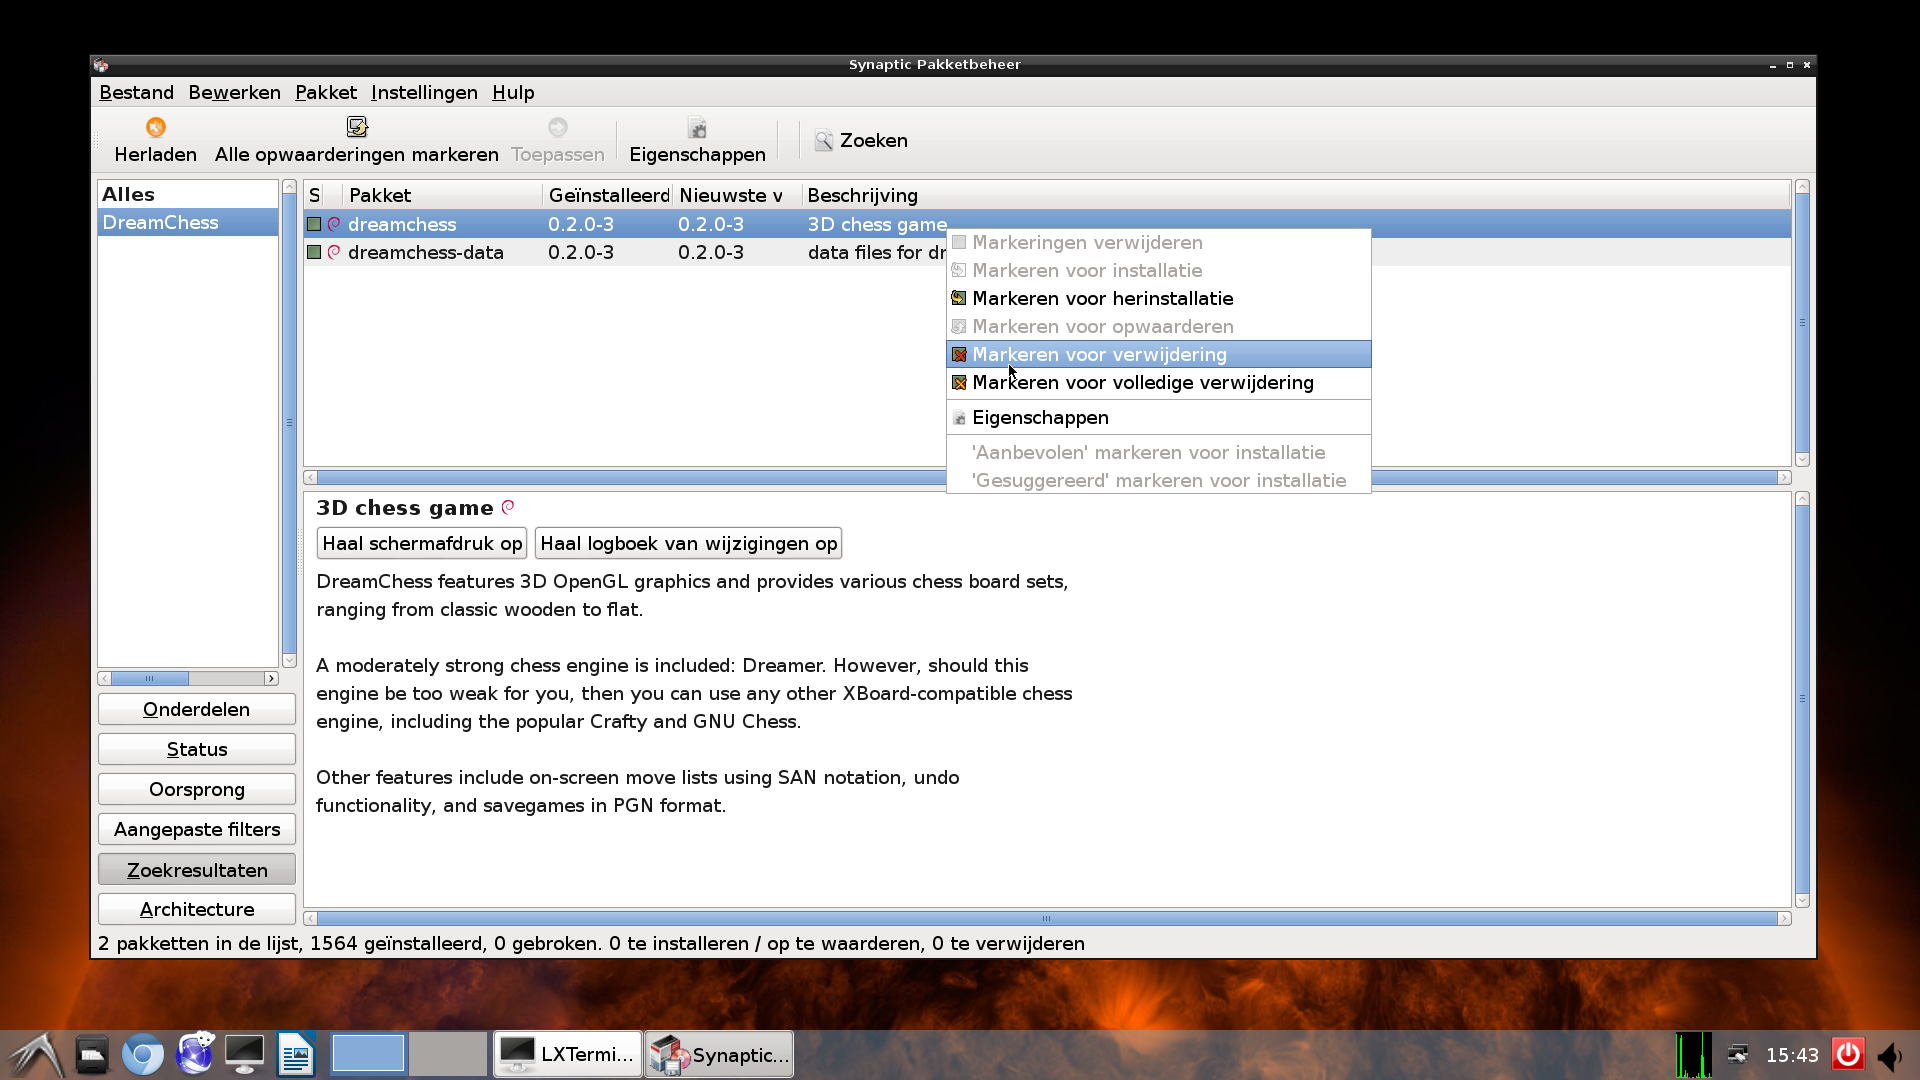
\includegraphics[width=0.45\textwidth]{plaatje16}
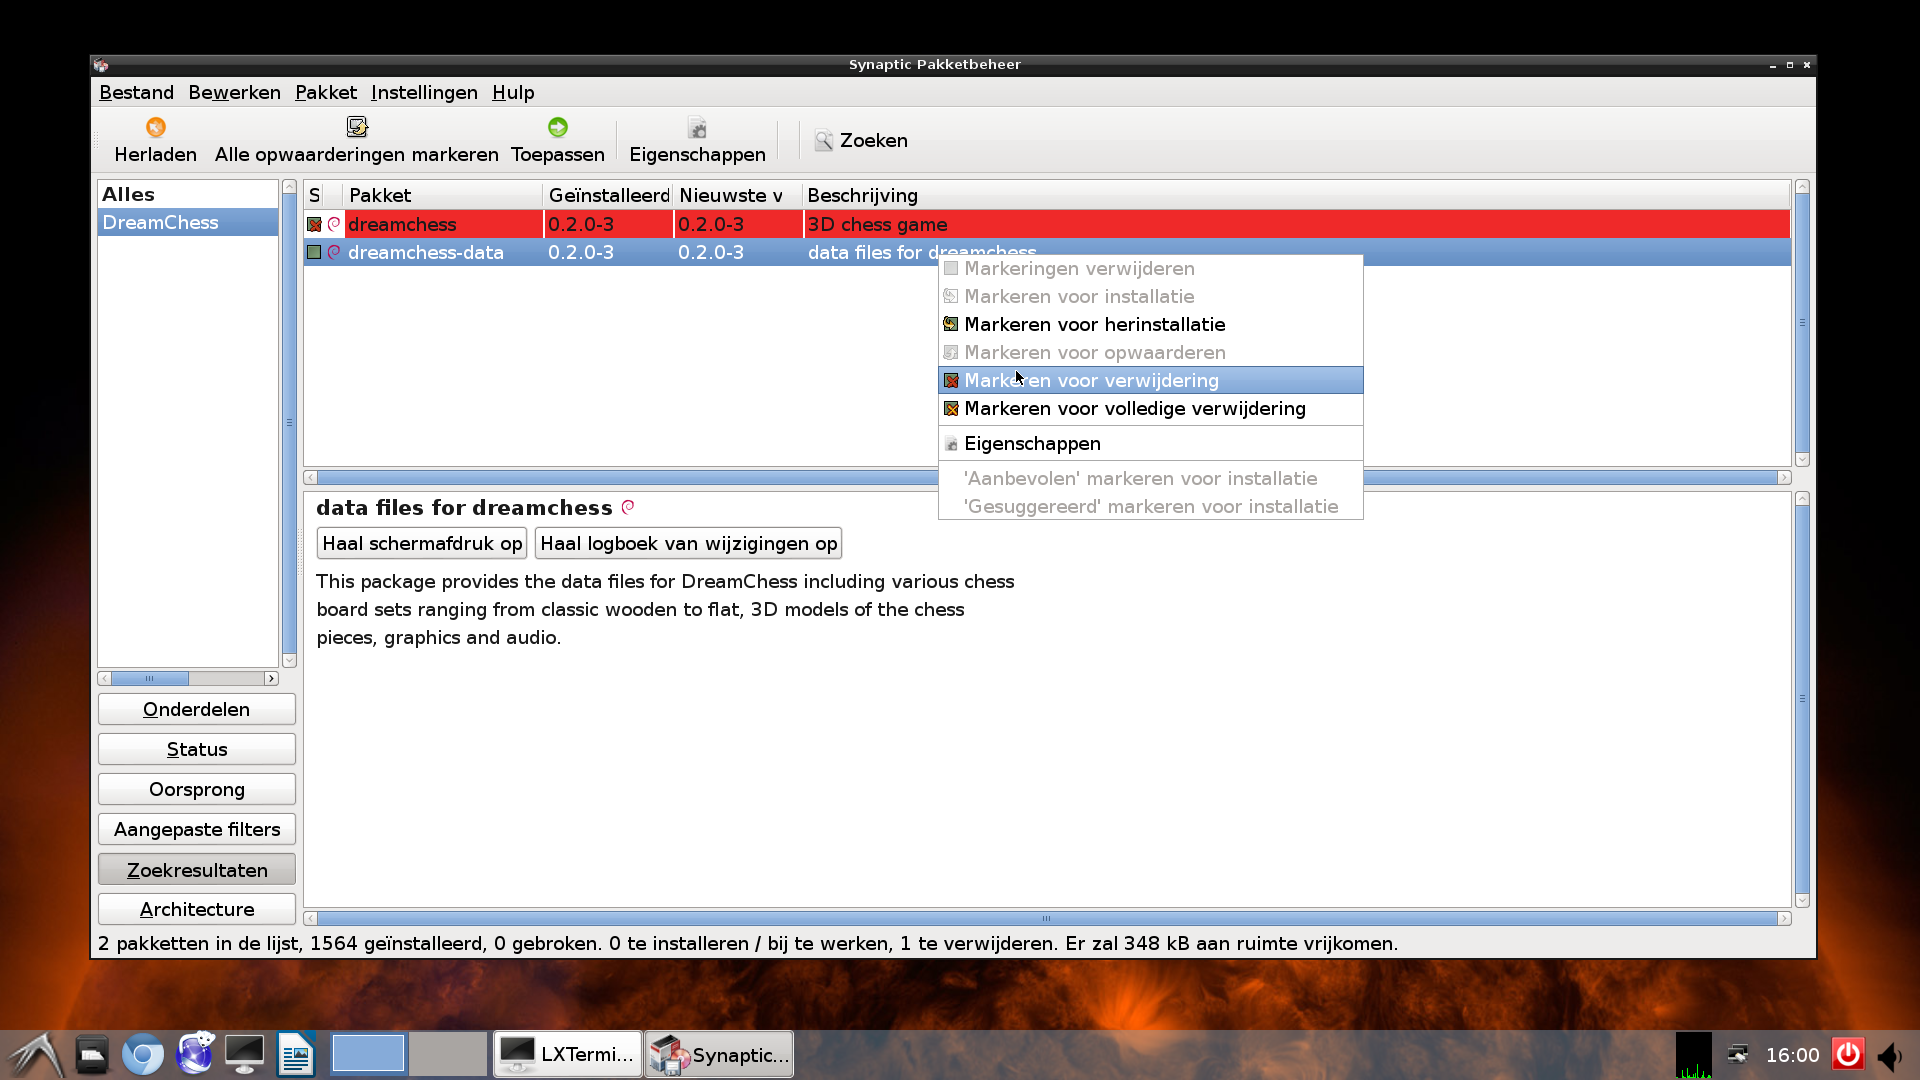
\includegraphics[width=0.45\textwidth]{plaatje17}
\caption{Markeren voor verwijdering}
\label{plaatje16}
\end{figure}

\noindent Een overzicht van de afhankelijkheden kun je bekijken onder de tab \emph{Eigenschappen}.  

\begin{figure} [H]
\centering
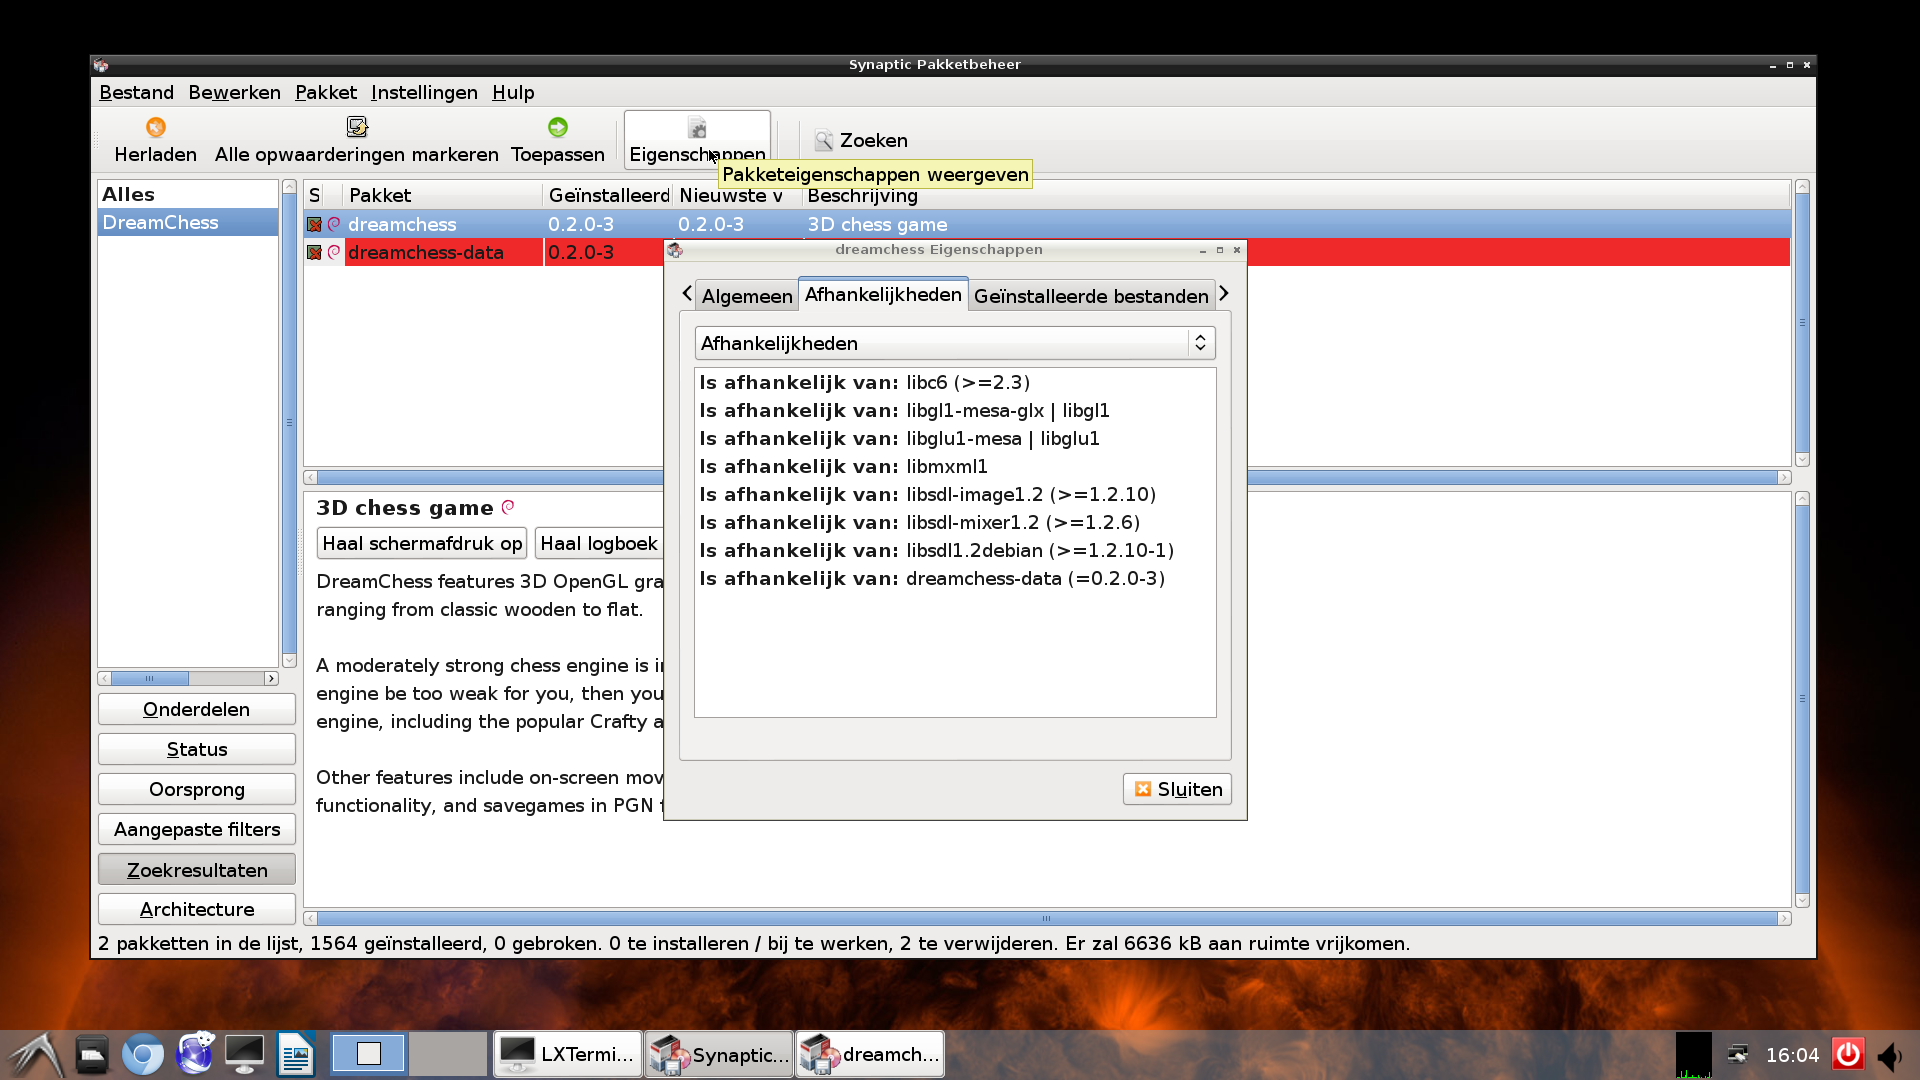
\includegraphics[width=0.6\textwidth]{plaatje18}
\caption{Een overzicht van afhankelijkheden}
\label{plaatje18}
\end{figure}

\noindent Als je aangemerkt hebt wat je wilt verwijderen, kies je Toepassen. Synaptic vraagt nog eens om bevestiging.  

\begin{figure} [H]
\centering
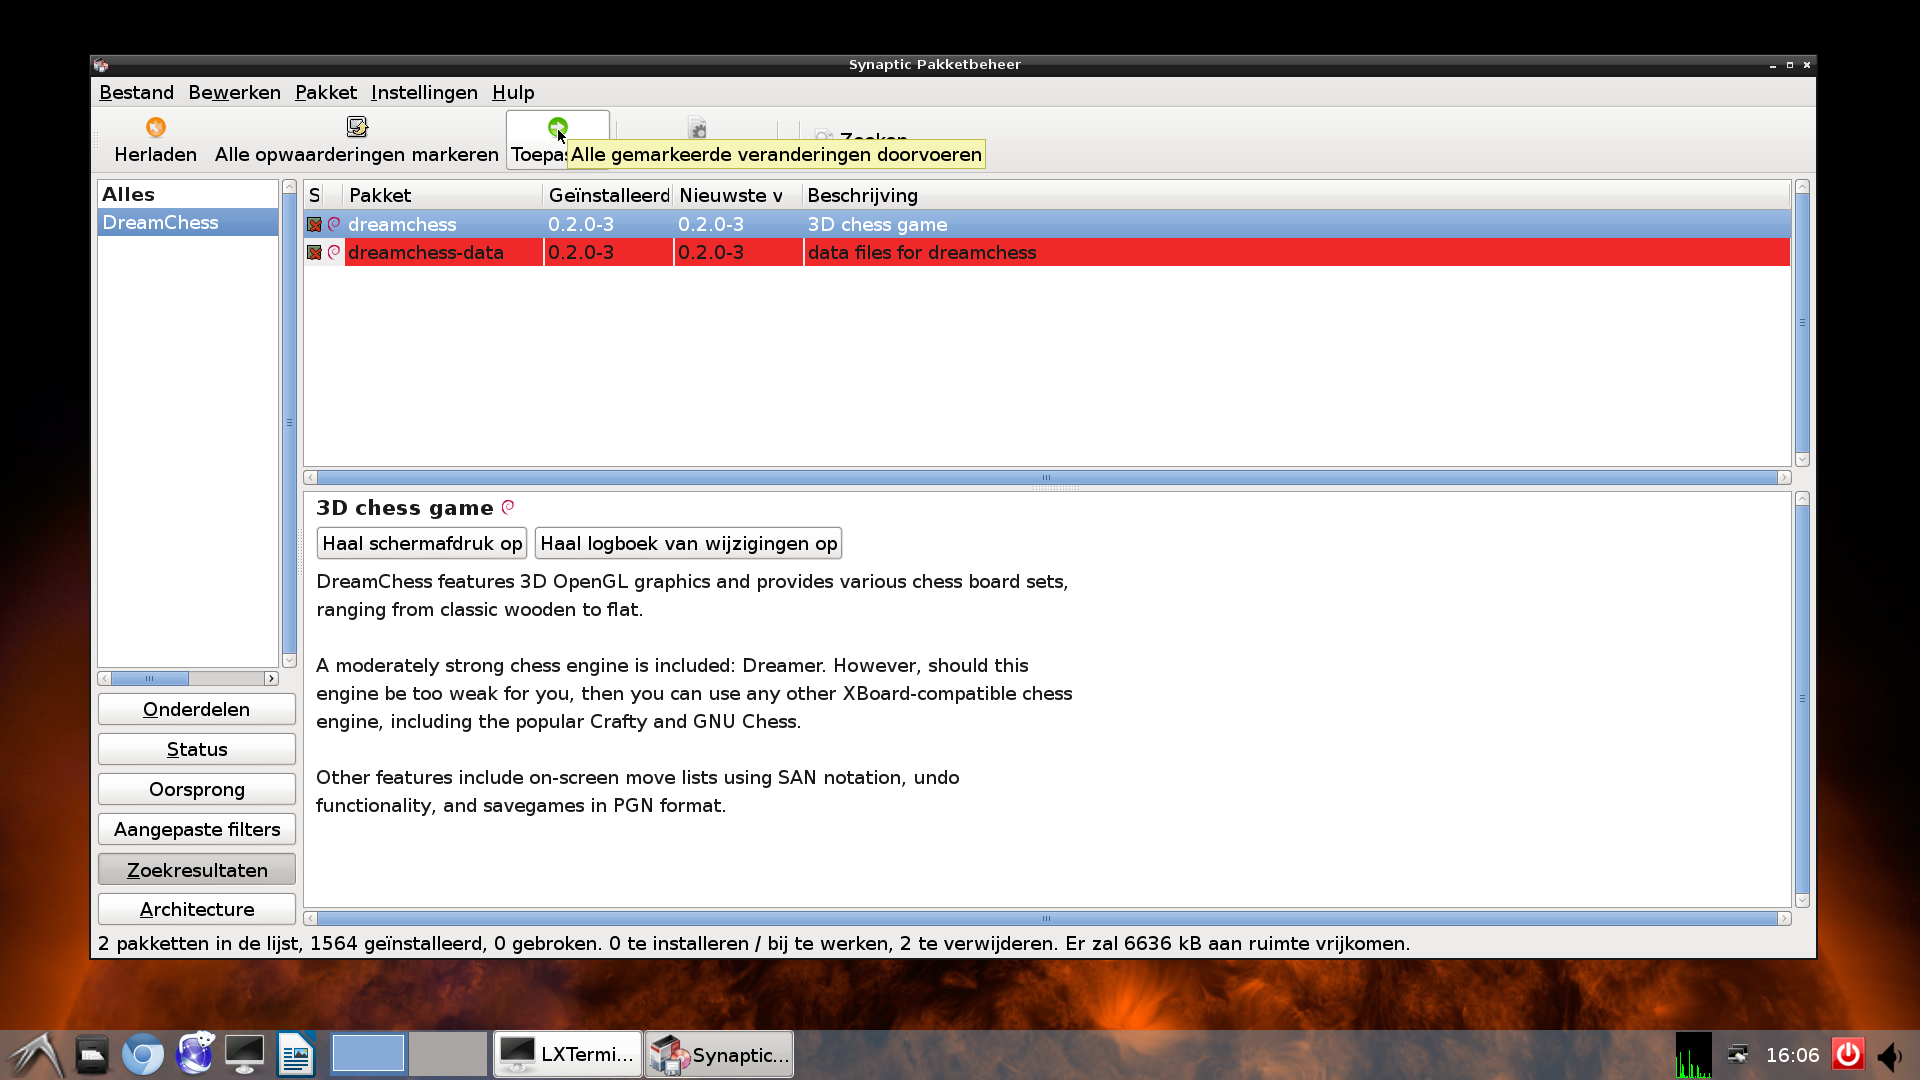
\includegraphics[width=0.45\textwidth]{plaatje19}
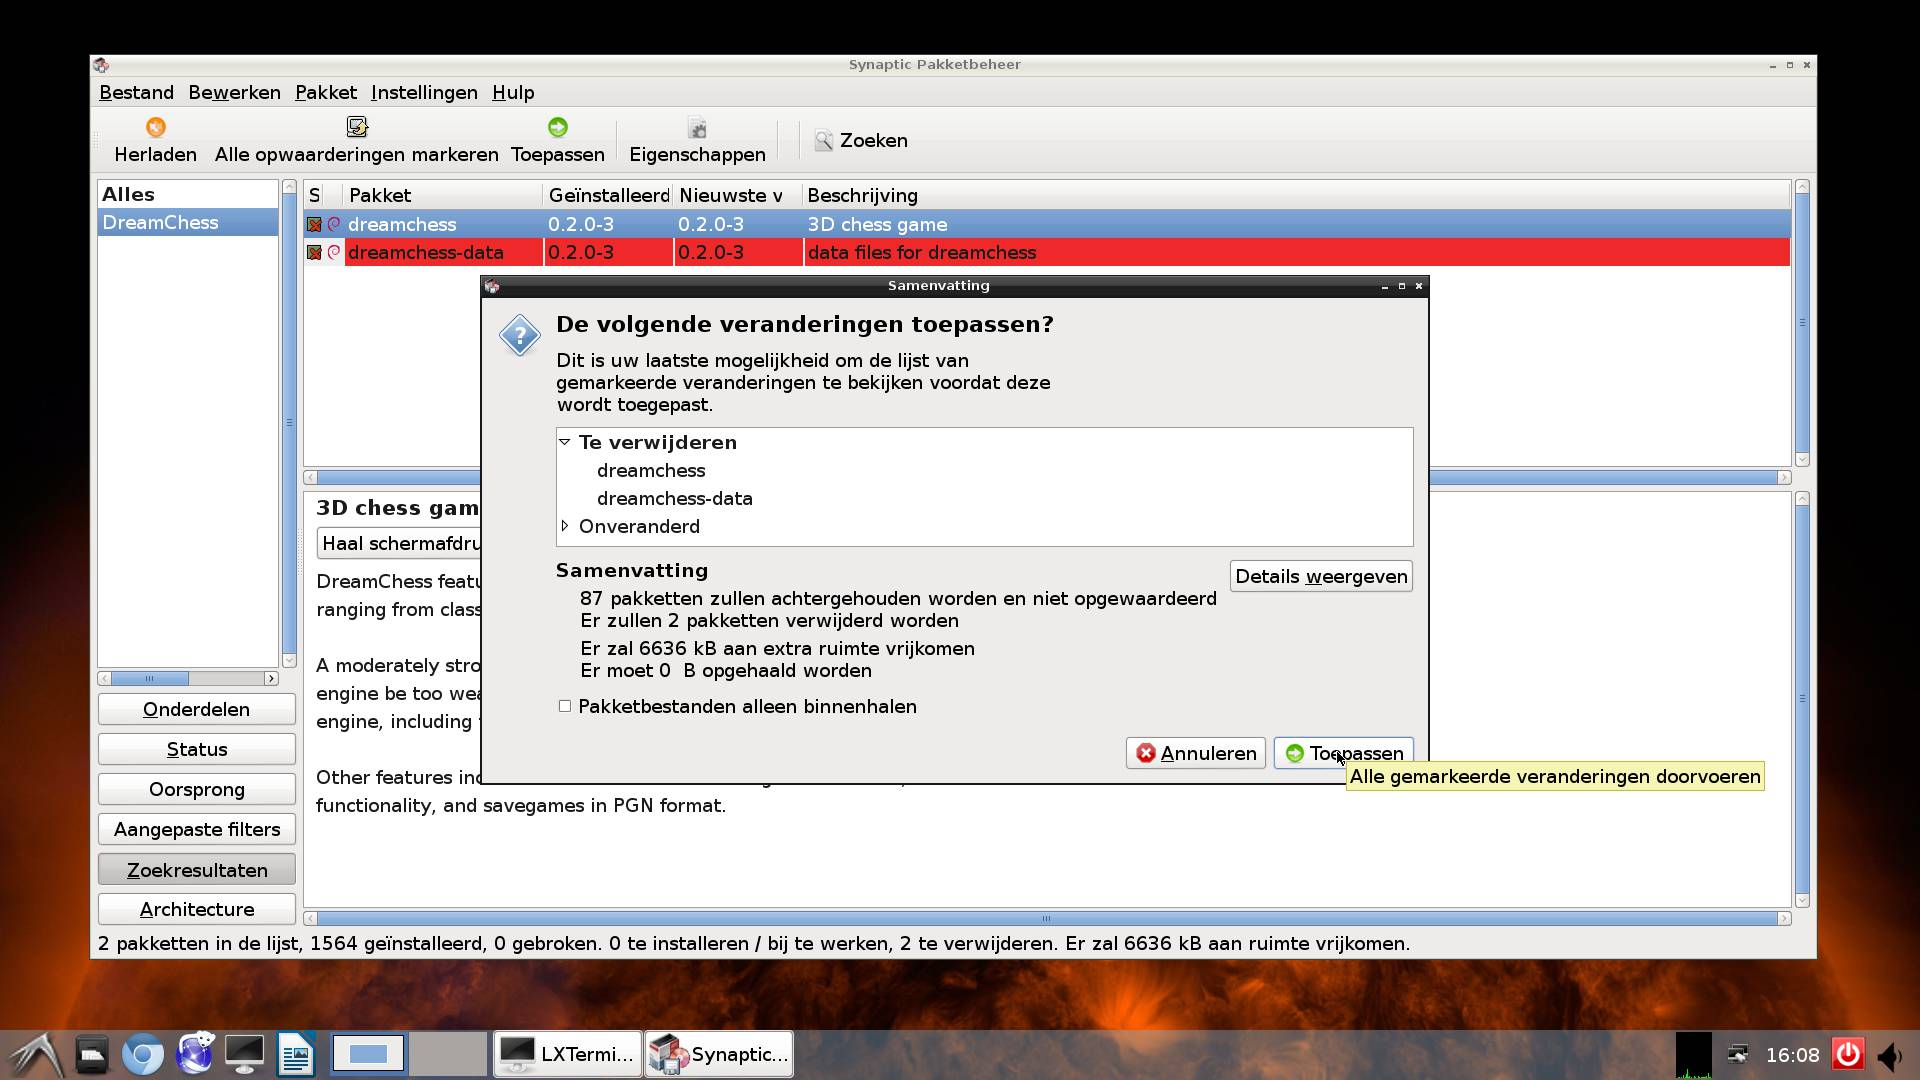
\includegraphics[width=0.45\textwidth]{plaatje20}
\caption{Veranderingen doorvoeren}
\label{plaatje19}
\end{figure}

\noindent Synaptic doet de rest. Je krijgt tot slot nog een venstertje ter bevestiging dat de de\"{i}nstallatie gelukt is.

\clearpage

\section{Voor gevorderden: de computer opschonen vanaf de terminal}

De terminal geeft je grote macht over je computer, en daarmee grote verantwoordelijkheid. Dus doe wat je durft, en doe niet wat je niet durft. OK?

Je opent LXTerminal. In het venster staat een tekstregel die lijkt op \texttt{gebruiker@computer~\$} . Op dezelfde regel voer je in:

\begin{lstlisting}[language=bash]
sudo apt-get autoremove
\end{lstlisting}

\noindent en doet enter. Je wordt nu gevraagd om je wachtwoord. Dat voer je in. Hierbij gebeurt er niets op het scherm. Je doet opnieuw enter. 

In het terminalvenster kun je nu volgen hoe de computer wordt opgeschoond. Als het proces is voltooid, kun je het venster sluiten. 
\vspace{1em}

\noindent \textbf{Wat is er nu gebeurd?} Met het commando \texttt{sudo} heb je gevraagd om beheersbevoegdheid om veranderingen aan te brengen in de computer. \texttt{sudo} vraagt altijd om je wachtwoord. Je gebruikt \texttt{sudo} all\'{e}\'{e}n als je weet wat je doet. Serieus. 

\texttt{apt-get} is het ``onzichtbare'' \textit{backend-}programma voor het installeren van programma's en het  aanbrengen van veranderingen aan ge\"{i}nstalleerde programma's. Aptitude is een voorkant voor \texttt{apt-get} en nog een paar van zulke scripts. \texttt{autoremove} was wat je \texttt{apt-get} vroeg om te doen. Daarmee zijn alle pakketten verwijderd waar geen andere programma's meer van afhankelijk zijn.

\end{document}
